


%% refer q31.tex
%% include the topic name as per u r project in appendix
\chapter{Block Diagram and Components Details}

\section{Block Diagram}

	\begin{figure}[h]
		\centering
	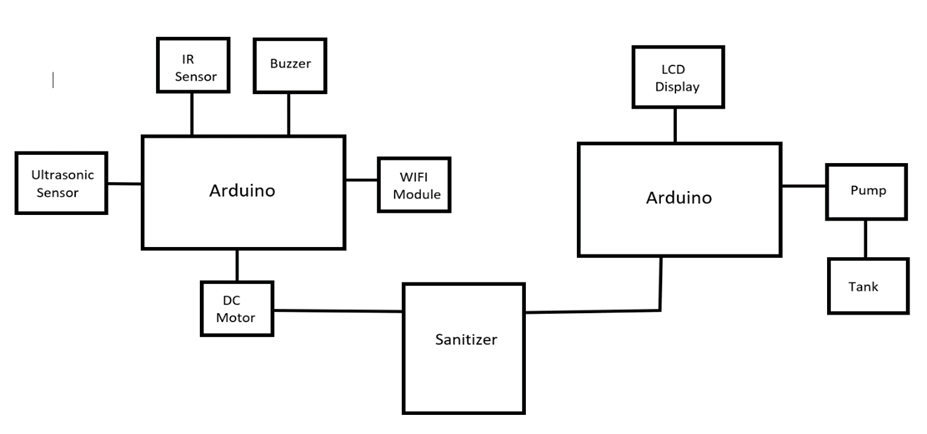
\includegraphics[width=140mm,scale=1]{50}
	\caption{Block Diagram}
	\label{Block Diagram}
	\end{figure}

    In this project we will use two Arduinos. Ultrasonic Sensor will connect to the Arduino and also DC Motor connect to the Arduino using motor driver IC. Other part of motor will connect to sanitizer bottle. IR Sensor and Buzzer also connect to same Arduino. Then we will connect WIFI module with Arduino.
	After that we will use second Arduino for automatic tank filling system. Pump will connect to that Arduino by using relay module. Other part of pump will connect to the tank. LCD display will also connect to the Arduino for indicating purpose. This Arduino will connect to sanitizer bottle by using probs.


\section{Components Details}
 \begin{itemize}
 	\item \Large\textbf {Arduino}
\end{itemize}
 
	\begin{figure}[h]
		\centering
	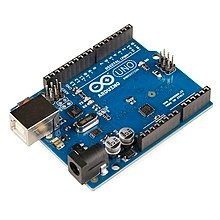
\includegraphics[width=60mm,scale=1]{41}
	\caption{Arduino Uno}
	\label{Arduino}
	
\end{figure}
 
 Arduino is an open-source platform used for building electronics projects. Arduino consists of both a physical programmable circuit board (often referred to as a microcontroller) and a piece of software, or IDE (Integrated Development Environment) that runs on your computer, used to write and upload computer code to the physical board. The Arduino platform has become quite popular with people just starting out with electronics, and for good reason. Unlike most previous programmable circuit boards, the Arduino does not need a separate piece of hardware (called a programmer) in order to load new code onto the board you can simply use a USB cable. Additionally, the Arduino IDE uses a simplified version of C++, making it easier to learn to program. Arduino uno has 14 digital input/output pins (of which 6 can be used as PWM outputs), 6 analog inputs, a USB connection, a power jack, a reset button and more. It contains everything needed to support the microcontroller; simply connect it to a computer with a USB cable or power it with a AC-to-DC adapter or battery.
 
\begin{itemize}
 	\item \Large\textbf {Bolt WIFI Module}
 \end{itemize}
 
	\begin{figure}[h]
		\centering
	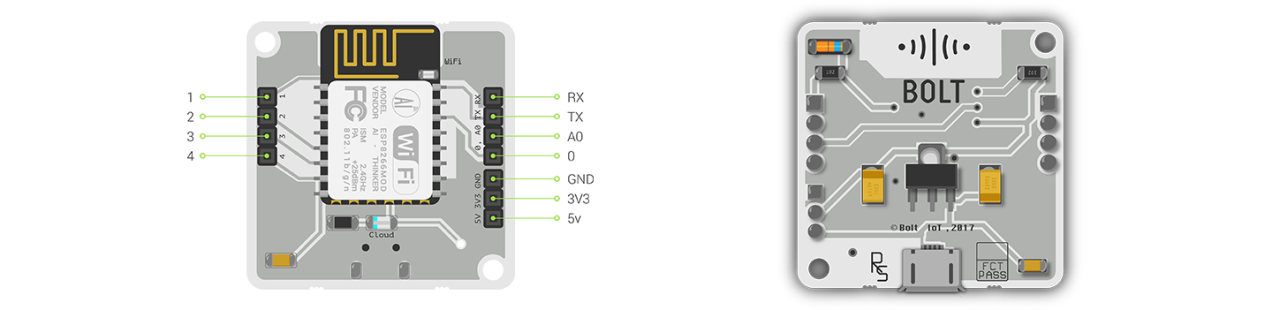
\includegraphics[width=120mm,scale=1]{42}
	\caption{Bolt WIFI Module}
	\label{Bolt WIFI Module}
	
\end{figure}

 The bolt Wifi module contains ESP8266 Wifi module. The ESP8266 Wifi Module is a self-contained SOC with integrated TCP/IP protocol stack that can give any microcontroller access to your Wifi network. The ESP8266 is capable of either hosting an application or offloading all Wi-Fi networking functions from another application processor. The ESP8266 module is an extremely cost effective board. This module has a powerful enough on-board processing and storage capability that allows it to be integrated with the sensors and other application specific devices through its GPIOs with minimal development up-front and minimal loading during runtime. Its high degree of on-chip integration allows for minimal external circuitry, including the front-end module, is designed to occupy minimal PCB area.
 
\newpage
\begin{itemize}
 	\item \Large\textbf {HC-SR04 Ultrasonic Sensor}
 \end{itemize}
 
	\begin{figure}[h]
		\centering
	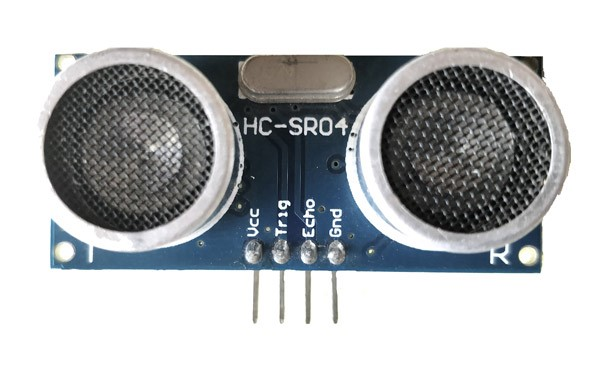
\includegraphics[width=60mm,scale=1]{43}
	\caption{HC-SR04 Ultrasonic Sensor}
	\label{HC-SR04 Ultrasonic Sensor}
	
\end{figure}

 The HC-SR04 ultrasonic sensor uses SONAR to determine the distance of an object just like the bats do. It offers excellent non-contact range detection with high accuracy and stable readings in an easy-to-use package from 2 cm to 400 cm or 1” to 13 feet.  It comes complete with ultrasonic transmitter and receiver module. Operating voltage: +5V  Theoretical Measuring Distance: 2cm to 450cm. Practical Measuring Distance: 2cm to 80cm.
 
\newpage
\begin{itemize}
 	\item \Large\textbf {IR Sensor}
 \end{itemize}
 
	\begin{figure}[h]
		\centering
	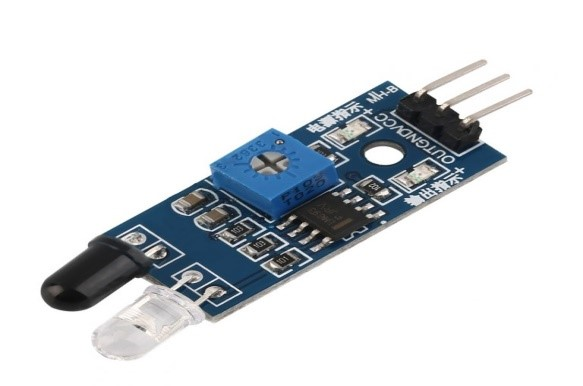
\includegraphics[width=60mm,scale=1]{44}
	\caption{IR Sensor}
	\label{IR Sensor}
	
\end{figure}

 IR sensor is an electronic device, that emits the light in order to sense some object of the surroundings. An IR sensor can measure the heat of an object as well as detects the motion. Usually, in the infrared spectrum, all the objects radiate some form of thermal radiation. These types of radiations are invisible to our eyes, but infrared sensor can detect these radiations. The emitter is simply an IR LED (Light Emitting Diode) and the detector is simply an IR photodiode . Photodiode is sensitive to IR light of the same wavelength which is emitted by the IR LED. When IR light falls on the photodiode, the resistances and the output voltages will change in proportion to the magnitude of the IR light received.
 
\newpage 
\begin{itemize}
 	\item \Large\textbf {Buzzer}
 \end{itemize}   
  
	\begin{figure}[h]
		\centering
	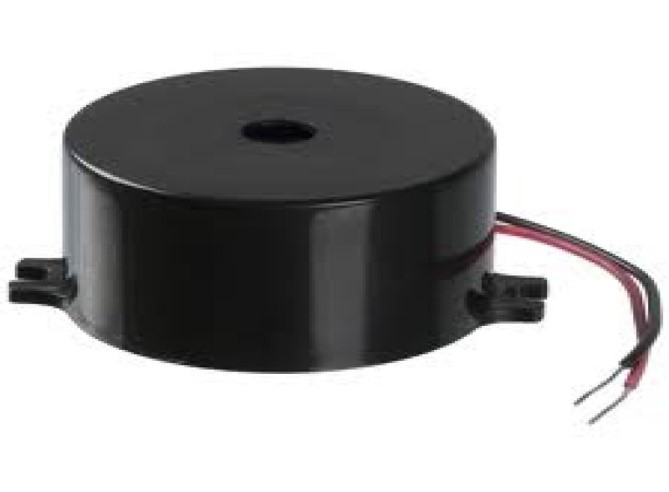
\includegraphics[width=60mm,scale=1]{45}
	\caption{Buzzer}
	\label{Buzzer}
	
\end{figure}

 A buzzer or beeper is an audio signalling device, which may be mechanical, electromechanical, or piezoelectric (piezo for short). Typical uses of buzzers and beepers include alarm devices, timers, and confirmation of user input such as a mouse click or keystroke.  
 
\newpage
\begin{itemize}
 	\item \Large\textbf {LCD Display}
 \end{itemize}
 
	\begin{figure}[h]
		\centering
	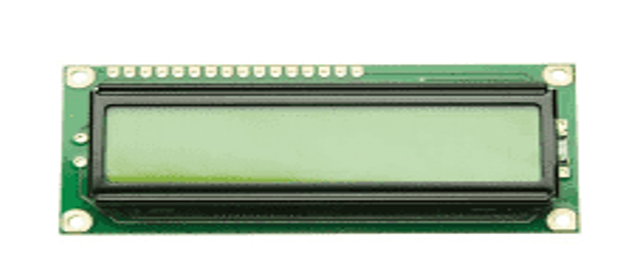
\includegraphics[width=60mm,scale=1]{46}
	\caption{LCD Display}
	\label{LCD Display}
	
\end{figure}

 LCD (Liquid Crystal Display) is a type of flat panel display which uses liquid crystals in its primary form of operation. LEDs have a large and varying set of use cases for consumers and businesses, as they can be commonly found in smartphones, televisions, computer monitors and instrument panels.
 
 
 \begin{itemize}
 	\item \Large\textbf {Stepper motor}
 \end{itemize}
 
	\begin{figure}[h]
		\centering
	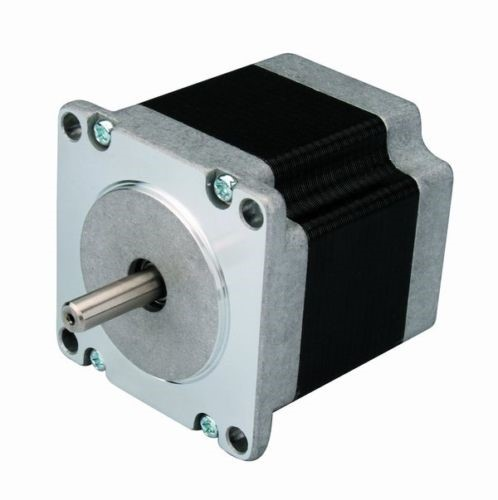
\includegraphics[width=60mm,scale=1]{47}
	\caption{Stepper Motor}
	\label{Stepper Motor}
	
\end{figure}

 The stepper motor is used for precise positioning with a motor, such as hard disk drives, robotics, antennas, telescopes, and some toys. Stepper motors cannot run at high speeds, but have a high holding torque. Stepper motors themselves function as ac motors. Stepper motors have a high pole count, usually between 50 and 100.
 
\newpage